%==================================================================
%  MEAM 6230  Final Project Report  -  Yicong Wang
%  Compile:  pdflatex final_report.tex (twice for refs)
%==================================================================
\documentclass[10pt,conference]{IEEEtran}

\usepackage[margin=0.75in]{geometry}
\usepackage[T1]{fontenc}
\usepackage{amsmath,amssymb,amsthm}
\usepackage{graphicx}
\usepackage{booktabs}
\usepackage{algorithm}
\usepackage{algpseudocode}
\usepackage{float}
\usepackage{hyperref}
\usepackage{cite}
\usepackage{xcolor}
\usepackage{bm}
\usepackage{multirow}
\usepackage{xurl}  

\definecolor{linkpink}{HTML}{C71585}   % VPP-TC paper 那种紫红色

\hypersetup{
    colorlinks=true,
    linkcolor=blue,
    citecolor=blue,
    urlcolor=linkpink,
}


\newcommand{\R}{\mathbb{R}}
\newcommand{\bx}{\bm{x}}
\newcommand{\bq}{\bm{q}}
\newcommand{\bdq}{\dot{\bm{q}}}
\newcommand{\bddq}{\ddot{\bm{q}}}
\newcommand{\btau}{\bm{\tau}}
\newcommand{\bM}{\bm{M}}
\newcommand{\bMt}{\widetilde{\bm{M}}}
\newcommand{\bh}{\bm{h}}
\newcommand{\bht}{\widetilde{\bm{h}}}
\newcommand{\bA}{\bm{A}}
\newcommand{\bP}{\bm{P}}
\newcommand{\norm}[1]{\left\lVert #1 \right\rVert}

\newtheorem{theorem}{Theorem}
\newtheorem{assumption}{Assumption}
\newtheorem{lemma}{Lemma}
\theoremstyle{remark}
\newtheorem{remark}{Remark}
\theoremstyle{plain}

\title{Safe Reactive Robot Control via\\ Viability-Preserving
Passive Torque Control}

\author{\IEEEauthorblockN{Yicong Wang}
\IEEEauthorblockA{
University of Pennsylvania\\
\texttt{yicongw@seas.upenn.edu}}}

\begin{document}
\maketitle

%==================================================================
\begin{abstract}
We extend Viability-Preserving Passive Torque Control
(VPP-TC)~\cite{zhang2025vpptc} along three coupled axes.
First, we expose a planner-agnostic interface and validate that
the safety layer accepts any globally asymptotically stable (GAS)
dynamical system as the upstream planner; we instantiate it with a
hand-drawn six-component LPV-DS~\cite{figueroa2018lpvds}.
Second, we re-derive the viability acceleration bounds under a
bounded inertial mismatch
$\norm{\Delta\bM\,\bM^{-1}}_2 \le \delta$ and introduce an
$\varepsilon$-margin that preserves viability for the entire
perturbation ball.
Third, whenever the upstream planner admits a quadratic Lyapunov
function---which includes both the original VPP-TC linear
attractor and a Hurwitz-projected LPV-DS as special cases---we
compose this Lyapunov function with the $\varepsilon$-tightened
QP to obtain an Input-to-State-Stability (ISS) bound on the
closed-loop tracking error, certifying practical convergence.
We port the framework, with no controller retuning, from the
single-arm Franka Panda to the Panda dual-arm and to the
Enactic OpenArm humanoid (both 14-DoF).
On 5 head-to-head scenarios, VPP-TC is self-collision free in
$5/5$ runs versus $2/5$ for a passivity-only baseline; on 96
high-uncertainty mass-mismatch cells the safety fallback prevents
$5$ otherwise-occurring self-collisions, while on a 24-cell
$\varepsilon$-margin sweep we observe and explain why the
margin's empirical value is regime dependent.
A final 17-cell sweep stress-tests Theorem~1 with the more
demanding mixture planner (LPV-DS) under mass mismatch
$p\in\{0,10,\dots,50\}\%$ and shows that the
practical-convergence ball predicted by the ISS analysis is
observed in simulation; the same theorem already covers the
linear planner used in the earlier sweeps.

{\sloppy\noindent\textit{Code:} \url{https://github.com/yicongw/meam623_final}\\
\textit{Videos:} \url{https://drive.google.com/drive/folders/1l37lh3_mBUwYNHC6a13PMtLwFM5gLA2c?usp=drive_link}\par}
\end{abstract}


%==================================================================
\section{Introduction}
\label{sec:intro}

Safe physical interaction between robots and humans demands two
properties \emph{simultaneously}: \emph{passivity}, so that energy
is strictly dissipated in unmodeled contacts, and \emph{viability},
so that hard constraints (joint limits, self- and external
collisions) are never violated.  Classical passive DS-tracking
controllers~\cite{kronander2016passive} guarantee the former by
closing an energy-tank loop around the DS-driven impedance
controller, but they treat safety as the responsibility of the
upstream DS shape; constraint enforcement is not part of the
controller. CPIC~\cite{zhang2024cpic} brings constraints into the
loop by constraining a DS-based impedance law with a
\emph{relaxed hierarchical CBF--QP} subject to multiple
(possibly contradicting) constraints derived from data-driven $C^2$
collision-boundary functions, and is ``passive only when feasible'';
in the contradictory regime the slack relaxation can momentarily
sacrifice strict passivity. The recently proposed
Viability-Preserving Passive Torque Control
(VPP-TC)~\cite{zhang2025vpptc} keeps both properties strict by
pre-computing analytical or learned viability sets in the
position-velocity state space and converting their boundaries into
cheap acceleration-level (and hence torque-level) bounds inside a
small QP, with a strictly dissipative fallback whenever those
bounds become infeasible.

\paragraph*{Goal} The goal of this project is to broaden VPP-TC
into a planner-agnostic, theoretically certified, multi-platform
safe-control framework: (i) decouple the safety layer from the
specific upstream planner so that any GAS dynamical system can
drive it; (ii) make the viability bounds robust to inertial model
mismatch with a quantitative margin; and (iii) prove that, under
this margin, safety \emph{and} practical convergence to the
planner's attractor hold simultaneously. The three contributions
below operationalise these three sub-goals.

\paragraph*{Contributions} This project investigates three
extensions of VPP-TC, all situated within the dynamical-systems
(DS) lens of motion planning and control studied in the course:
\begin{itemize}
    \item[(C1)] \textbf{Planner-agnostic interface and
        multi-platform porting.} We replace the single-arm linear
        attractor with a hand-drawn $K{=}6$ LPV-DS and port the
        full pipeline---without re-tuning---to the Franka Panda
        dual-arm and to the OpenArm humanoid (both 14-DoF).
    \item[(C2)] \textbf{$\varepsilon$-margin under inertial
        mismatch.} We derive an $\varepsilon$ tightening of the
        viability bounds that restores feasibility for the whole
        perturbation ball, and we measure its limits empirically.
    \item[(C3)] \textbf{Unified safety + convergence.} Whenever the
        upstream planner $f$ is GAS at $\bx^\star$ with a quadratic
        Lyapunov function $V(\bx)$---in particular, both the
        original VPP-TC linear attractor and any Hurwitz-projected
        LPV-DS---the $\varepsilon$-tightened VPP-TC closed loop is
        ISS in the mismatch level $\delta$, with a finite
        practical-convergence ball whose radius scales with
        $\delta$ (Theorem~\ref{thm:iss}).
\end{itemize}

We treat (C2) and (C3) as the main technical thread of the
project: we first observe empirically that, under the proposal's
default mismatch sweep, ``the safety fallback secures collision
freedom but stalls $30$--$80$\,cm short of the target''
(Sec.~\ref{sec:exp-fallback}); the $\varepsilon$-margin restores
QP feasibility so the controller follows the planner instead of
the dissipative fallback, and composing the planner's quadratic
Lyapunov function with the bounded controller-tracking error
yields the quantitative convergence guarantee
(Sec.~\ref{sec:exp-unified}).

%==================================================================
\section{Related Work}

\paragraph*{Passive DS tracking}  Kronander and
Billard~\cite{kronander2016passive} close an energy-tank loop
around a DS-tracking impedance controller so that the closed loop
is passive even when the DS is non-conservative. The architecture
is concerned with passivity, not with hard kinematic or
self-collision constraints; the safety profile of the resulting
behavior is inherited entirely from the DS that the user supplies.

\paragraph*{CBF and viability}  Ames~\cite{ames2019cbf} popularized
CBF-QPs that enforce forward invariance of a safe set. Viability
theory~\cite{aubin1991viability} is the larger framework that asks
which states admit a control trajectory keeping the system inside
the constraint set indefinitely; CBFs are essentially a smooth
sub-class of viability boundaries. A complementary line of work
learns CBFs from data: So et al.~\cite{so2024neuralcbf} construct
a Policy Neural CBF (PNCBF) by learning the value function of a
nominal policy under the maximum-over-time cost, which is then
used as a CBF for systems with high relative degree and input
constraints. VPP-TC takes a different route: rather than fitting a
smooth CBF, it learns a binary self-collision predictor
(TransformerGamma) and converts its level-set boundary directly
into an acceleration-level viability bound.

\paragraph*{Passive Interactive Control with hard constraints}
CPIC~\cite{zhang2024cpic} constrains a DS-based impedance law with
a relaxed hierarchical CBF--QP subject to multiple, possibly
contradicting, constraints derived from data-driven $C^2$
self- and external-collision boundary functions; the controller is
``passive only when feasible'', i.e.\ strict passivity may be
sacrificed via slack when constraints conflict. VPP-TC instead
bakes the safety constraint into a torque-passive QP and falls
back to a strictly dissipative brake \eqref{eq:fallback} whenever
the constraints become infeasible; the
$\varepsilon$-margin~(\S\ref{sec:eps-margin}) is what we tune to
keep that fallback rare under inertial mismatch.

\paragraph*{LPV-DS planning}  LPV-DS planners fit a mixture of
linear systems with shared Hurwitz constraints to expert
demonstrations~\cite{figueroa2018lpvds}; the resulting field is
continuously differentiable and admits a common quadratic
Lyapunov function, which is the only structure our convergence
proof needs. More general DS-stability frameworks---\emph{e.g.}\
learned control-Lyapunov functions without the quadratic
restriction~\cite{khansari2014clf}---also satisfy the hypothesis
of Theorem~\ref{thm:iss}, but the quadratic case suffices for
this work.

%==================================================================
\section{Preliminaries}
\label{sec:back}

\subsection{Robot dynamics and the nominal QP controller}
For an $n$-link manipulator with configuration $\bq\in\R^n$, the
true rigid-body dynamics are
\begin{equation}
    \bMt(\bq)\,\bddq + \bht(\bq,\bdq) = \btau,
    \label{eq:dyn-true}
\end{equation}
while the controller is built on the nominal model
$\bM(\bq),\,\bh(\bq,\bdq)$. Define the inertial mismatch
$\Delta\bM = \bMt - \bM$ and assume
\begin{equation}
    \norm{\Delta\bM(\bq)\,\bM(\bq)^{-1}}_2 \le \delta
    \quad \forall\,\bq.
    \label{eq:delta-bound}
\end{equation}

The VPP-TC controller computes an end-effector command
$\bx^d=f(\bx)$ from the upstream DS planner, maps it to a desired
joint acceleration $\bddq^{\text{des}} = \bddq^{\text{des}}(\bx,
\bdq, f(\bx))$, and solves a small QP that returns a passive
torque while staying within the viability bounds:
\begin{equation}
\begin{aligned}
\btau^* = \arg\min_{\btau}\;
    & \norm{\bM^{-1}(\btau-\bh) - \bddq^{\text{des}}}_2^2
      + \alpha\norm{\btau}_2^2 \\
\text{s.t.}\quad
    & \bddq^{\min}(\bq,\bdq) \le \bM^{-1}(\btau-\bh)
                            \le \bddq^{\max}(\bq,\bdq), \\
    & L_f h_{\Gamma} + L_g h_{\Gamma}\,\bM^{-1}(\btau-\bh)
                            + \alpha_{\Gamma} h_{\Gamma} \ge 0,
\end{aligned}
\label{eq:vpptc-qp}
\end{equation}
where $\bddq^{\min},\bddq^{\max}$ are joint-limit and
self-collision viability bounds, and $h_\Gamma(\bq)$ is the
TransformerGamma collision predictor of~\cite{zhang2025vpptc}.

If the QP is infeasible (which happens whenever the constraint
intersection is empty under the \emph{nominal} model), VPP-TC
falls back to
\begin{equation}
    \btau^{\text{fbk}} = \bh(\bq,\bdq) - \bm{K}\bdq,
    \label{eq:fallback}
\end{equation}
i.e.\ gravity/Coriolis compensation plus viscous damping on $\bdq$.
This is a strictly dissipative (passive) brake; it does not
contain a target term and therefore cannot drive the end-effector
to the goal, but it guarantees energy decay.

\subsection{LPV-DS as the high-level planner}
A linear-parameter-varying DS (LPV-DS) is a soft mixture of
linear flows
\begin{equation}
    f(\bx) = \sum_{k=1}^K \gamma_k(\bx)\bigl(\bA_k\bx + \bm{b}_k\bigr),
    \quad \sum_k \gamma_k(\bx)=1,
    \label{eq:lpvds}
\end{equation}
with $\gamma_k(\bx)\in[0,1]$ a smooth membership weight (we use a
Gaussian mixture). When fitted with the
Hurwitz constraint $\bA_k+\bA_k^\top\prec 0$ and a shared
attractor $\bx^\star$, $f$ admits a common quadratic Lyapunov
function $V(\bx)=(\bx-\bx^\star)^\top \bP (\bx-\bx^\star)$ for any
$\bP\succ 0$ that is co-feasible with all $\bA_k$~\cite{figueroa2018lpvds},
and is \emph{globally asymptotically stable} at $\bx^\star$.

%==================================================================
\section{Method: VPP-TC with an $\varepsilon$-Margin and a
Quadratic-Lyapunov Planner}
\label{sec:method}

\subsection{Where the nominal QP \eqref{eq:vpptc-qp} fails}
Plugging the controller torque
$\btau^* = \bM\,\bddq^{\text{des}} + \bh + \bm{r}$ (with
$\bm{r}$ a small residual) into the true plant
\eqref{eq:dyn-true} yields the realised acceleration
\begin{align}
    \bddq^{\text{real}}
        &= \bMt^{-1}\bigl(\btau^* - \bht\bigr) \notag \\
        &= \bM^{-1}\bigl(\bI + \Delta\bM\,\bM^{-1}\bigr)^{-1}
            \bigl[(\btau^* - \bh) + (\bh-\bht)\bigr] \notag \\
        &= \bddq^{\text{des}} + \bm{e}(\bq,\bdq,\delta),
\end{align}
where $\norm{\bm{e}} \le c_1\delta\,\norm{\bddq^{\text{des}}}
+ c_2\delta\,\norm{\bdq}^2$ for problem-dependent
constants. Hence the nominal viability bounds
$\bddq^{\min},\bddq^{\max}$ may be violated by an amount of
order $\delta$ even when $\btau^*$ satisfies them under the
nominal model.

\subsection{The $\varepsilon$-margin}
\label{sec:eps-margin}
We tighten the QP's acceleration bounds by an additive margin
$\varepsilon\!\ge\!0$:
\begin{equation}
    \bddq^{\min} + \varepsilon\,\lvert\bddq^{\max}\rvert
    \le \bM^{-1}(\btau-\bh) \le
    \bddq^{\max} - \varepsilon\,\lvert\bddq^{\max}\rvert.
    \label{eq:eps-bounds}
\end{equation}
\begin{lemma}[Margin sufficiency]
\label{lem:margin}
If $\varepsilon \ge \delta\bigl(c_1 + c_2\norm{\bdq}^2/
                              \norm{\bddq^{\max}}\bigr)$
holds pointwise (with $c_1, c_2$ the constants of the
preceding error bound, and using $\norm{\bddq^{\text{des}}}\le
\norm{\bddq^{\max}}$ to absorb the $c_1$ term), then the realised
acceleration $\bddq^{\text{real}}$ satisfies the original
(un-tightened) bounds, hence the viability set is forward
invariant under the true dynamics.
\end{lemma}

The proof is by direct substitution of the bound on $\bm{e}$ and
is omitted for space.

\subsection{Unified safety-and-convergence theorem}
\label{sec:unified}
With the $\varepsilon$-margin in place, the QP
\eqref{eq:vpptc-qp} no longer destroys feasibility under
\eqref{eq:delta-bound}. We can then reason about convergence.

\begin{theorem}[Practical ISS convergence]
\label{thm:iss}
Let the upstream planner $f(\bx)$ be GAS at $\bx^\star$ and
admit a quadratic Lyapunov function
$V(\bx)=(\bx-\bx^\star)^\top \bP(\bx-\bx^\star)$ with $\bP\succ 0$
that decays at rate $\alpha>0$ along the unperturbed flow,
\emph{i.e.}\ $\dot V_{\!f}(\bx) \le -\alpha\, V(\bx)$ for all
$\bx$.
Let the inertial mismatch satisfy \eqref{eq:delta-bound} and let
the $\varepsilon$-margin satisfy Lemma~\ref{lem:margin}. Then
along closed-loop trajectories of \eqref{eq:vpptc-qp} the
end-effector tracking error satisfies
\begin{equation}
    \limsup_{t\to\infty}\,\norm{\bx(t)-\bx^\star}^2
    \;\le\; \frac{c_3 \delta^2}{\alpha\,\lambda_{\min}(\bP)}.
    \label{eq:iss-bound}
\end{equation}
Equivalently, taking square roots,
$\limsup_{t\to\infty}\norm{\bx(t)-\bx^\star}
 \le \sqrt{c_3/(\alpha\,\lambda_{\min}(\bP))}\,\delta$,
so the practical-convergence ball scales \emph{linearly} with the
mismatch level $\delta$ when measured in raw distance units.
\end{theorem}

\noindent\emph{Sketch.} Under Lemma~\ref{lem:margin} the QP is
feasible at every instant, so the realised end-effector velocity
is $\dot{\bx} = f(\bx) + \bm{w}(\bq,\bdq,\delta)$ with
$\norm{\bm{w}}\le c_3'\delta$.
Differentiating $V$ along the perturbed flow,
$\dot V \le -\alpha V + 2\norm{\bP}\norm{\bx-\bx^\star}\norm{\bm{w}}$,
and a standard ISS argument~\cite[\S 4.9]{khalil2002nonlinear}
yields \eqref{eq:iss-bound}.\hfill$\square$

\begin{remark}[Concrete planners]
\label{rem:planners}
The hypothesis is satisfied by (i) the original VPP-TC linear
attractor $f(\bx)=\bA(\bx-\bx^\star)$ for any Hurwitz $\bA$,
where $\bP$ is the unique solution of the Lyapunov equation
$\bA^\top\bP+\bP\bA=-\bm Q$ for any chosen $\bm Q\succ 0$ and
$\alpha=\lambda_{\min}(\bm Q)/\lambda_{\max}(\bP)$;
and (ii) any Hurwitz-projected LPV-DS
\eqref{eq:lpvds}, where $\bP$ is the common solution of the
$K$-LMI system of \cite{figueroa2018lpvds} and
$\alpha=\min_k\lambda_{\min}(-\bA_k^\top\bP-\bP\bA_k)/\lambda_{\max}(\bP)$.
The linear case is the trivial $K{=}1$ instance; LPV-DS extends
the certificate to nonlinear demonstrations without changing the
proof.
\end{remark}

Theorem~\ref{thm:iss} is the main analytical contribution: it
replaces the ``fallback secures safety, convergence is not
guaranteed'' empirical statement of Sec.~\ref{sec:exp-fallback}
with a $\delta\!\to\!0$ recovery of the unperturbed convergence
behavior, mediated by the design parameter $\varepsilon$ via
Lemma~\ref{lem:margin}. The recovery mechanism is the
$\varepsilon$-margin keeping the QP feasible (so the controller
follows $f$ rather than the dissipative fallback); the planner
itself only needs to supply a quadratic Lyapunov object for the
proof to close.

\subsection{Algorithm summary}
Algorithm~\ref{alg:vpptc} packages the components of
Sec.~\ref{sec:method} into a single per-step routine. Line~2 is
the only call into the upstream DS, which is the
planner-agnostic interface from Contribution~(C1):
swapping the linear attractor for the LPV-DS leaves
lines~3--7 unchanged. Line~5 implements the
$\varepsilon$-tightening~\eqref{eq:eps-bounds} of
Contribution~(C2), and the QP/fallback split on line~6 is the
mechanism that makes Theorem~\ref{thm:iss} of Contribution~(C3)
operational: when the $\varepsilon$-margin keeps the QP feasible
the controller follows the planner and the ISS bound applies; when
it does not, \eqref{eq:fallback} preserves passivity at the cost
of progress.

\begin{algorithm}[H]
\caption{VPP-TC with $\varepsilon$-margin and quadratic-Lyapunov planner}
\label{alg:vpptc}
\begin{algorithmic}[1]
\Require nominal $\bM,\bh$; LPV-DS $\{\bA_k,\bm{b}_k,\gamma_k\}$,
attractor $\bx^\star$; viability oracle $h_\Gamma$, RDF SDF
$h_{\text{obs}}$; margin $\varepsilon$, gain $\alpha_\Gamma$.
\For{each control step}
  \State Read $(\bq,\bdq)$; compute $\bx$ via FK.
  \State $\bx^d \gets \sum_k \gamma_k(\bx)(\bA_k\bx+\bm{b}_k)$.
  \State $\bddq^{\text{des}}\gets J^{\dagger}(\bq)\bigl(K_d(\bx^d-\dot\bx)
       - \dot J\bdq\bigr)$.
  \State Compute viability bounds
     $(\bddq^{\min},\bddq^{\max})$ from $h_\Gamma,h_{\text{obs}}$.
  \State Tighten by $\varepsilon$ as in \eqref{eq:eps-bounds}.
  \State Solve QP \eqref{eq:vpptc-qp}; if infeasible apply
       \eqref{eq:fallback}.
  \State Send $\btau^*$ to robot.
\EndFor
\end{algorithmic}
\end{algorithm}

%==================================================================
\section{Experiments}
\label{sec:exp}

\subsection{Setup and metrics}
All experiments run in PyBullet with a fixed step
$h{=}2$\,ms (1\,ms for OpenArm). The TransformerGamma
self-collision model is the one shipped with~\cite{zhang2025vpptc};
we re-train it for the dual-arm and OpenArm topologies but keep
the architecture and training recipe unchanged. The QP
\eqref{eq:vpptc-qp} is solved with OSQP via
CVXPY~\cite{cvxpy,osqp}; the LPV-DS \eqref{eq:lpvds} is fit
on a hand-drawn 2D demonstration with $K{=}6$ Hurwitz components,
then lifted to 3D with an out-of-plane stiffness term.
We report: minimum self-collision distance
$d_{\text{sc}}^{\min}$, minimum learned predictor margin
$\Gamma^{\min}$, peak joint-velocity overshoot
$\dot q^{\text{over}}_{\max}$, percentage of steps in which the
soft fallback fires, and the final end-effector-to-target
distance $\norm{\bx(T)-\bx^\star}$.

% ----------------------------------------------------------------
\subsection{(C1a) Multi-platform porting at constant controller}
\label{sec:exp-porting}

We run the exact same Python module---no controller retuning, no
gain re-search---on three robots: a single-arm Franka Panda
(7-DoF), a Panda dual-arm (14-DoF), and the Enactic OpenArm
humanoid (14-DoF). The single-arm task is a fixed end-effector
reach; the dual-arm and OpenArm tasks are bilaterally crossing
limit cycles that deliberately bring the two end-effectors into
the same workspace patch.

The only platform-specific inputs are the URDF and a single
re-trained TransformerGamma weight file per topology; all
controller hyperparameters ($\varepsilon$, $\alpha_\Gamma$,
fallback gain $\bm K$, the QP regulariser) are unchanged across
all three robots. On every platform the viability filter keeps
the actual contact distance at PyBullet's contact-resolver noise
floor: across the full 6\,s rollouts the closest unsigned
distance returned by \texttt{getClosestPoints} stays below
$0.01$\,cm in absolute value, well inside PyBullet's resolver
tolerance ($\sim\!50\,\mu$m). On the dual OpenArm the
TransformerGamma surrogate (the smallest of the three, trained on
the fewest samples) briefly returned a mildly negative
$\hat{\gamma}_{\min}=-1.81$ during the most aggressive bimanual
approach; our soft-constraint relaxation absorbed this
conservative-prediction error without any actual inter-arm
penetration, illustrating that the QP layer is robust to
imperfect $\hat{\gamma}$ as long as the surrogate's sign is
roughly calibrated near contact.

We deliberately do not report a head-to-head wall-clock or
loop-rate comparison across the three platforms: control-loop
rates in our PyBullet harness are dominated by simulator stepping
and visualisation overhead rather than the controller itself, and
counter-intuitive cross-platform numbers (\emph{e.g.}\ a 14-DoF
dual arm appearing faster than a 7-DoF single arm) reflect
harness configuration rather than the controller. The qualitative
porting claim---one controller, three URDFs, no retuning, no
self-collisions---is what (C1a) asserts and is what we observe.

% ----------------------------------------------------------------
\subsection{(C1b) Head-to-head with a passivity-only baseline}
\label{sec:exp-baseline}

We compare VPP-TC with a passivity-only baseline (CFC), which
uses the same QP structure but with the viability and
self-collision constraints disabled. Five reach scenarios were
selected by an automatic search to expose the difference
(Sec.~\ref{sec:probe}).
Across $5/5$ scenarios VPP-TC remained self-collision-free
(min $d_{\text{sc}} = 0.9$\,cm in the worst case, on
\emph{base\_top}; still well above PyBullet's contact-resolver
floor), while the
passivity-only baseline self-collided in $3/5$ scenarios
(\emph{under\_arm}, \emph{under\_arm\_hi}, \emph{base\_top}).
Mean final tracking error was $0.84$\,cm for VPP-TC vs.\
$3.67$\,cm for CFC; in the
two scenarios where CFC remained collision-free
(\emph{near\_base}, \emph{snake}) both controllers reached
sub-millimeter accuracy. The full table is in
Table~\ref{tab:baseline}; the velocity-overshoot column shows
that CFC also exceeds $\dot q_{\max}$ by up to $3.0$\,rad/s in
the \emph{snake} scenario, which the joint-velocity term of the
VPP-TC bound suppresses.

\begin{table}[t]
\centering
\caption{VPP-TC vs.\ passivity-only baseline (CFC), 5 scenarios.
``SC'' marks self-collision; final dist.\ in cm.}
\label{tab:baseline}
\small
\begin{tabular}{@{}lccccc@{}}
\toprule
\multirow{2}{*}{Scenario}
       & \multicolumn{2}{c}{VPP-TC}
       & \multicolumn{2}{c}{Passivity-only (CFC)} \\
\cmidrule(lr){2-3}\cmidrule(lr){4-5}
       & SC? & final & SC? & final \\
\midrule
under\_arm    & no & $0.0$ & \textbf{yes} & $8.94$ \\
near\_base    & no & $0.0$ & no           & $0.0$  \\
under\_arm\_hi& no & $0.0$ & \textbf{yes} & $5.94$ \\
base\_top     & no & $4.19$ & \textbf{yes}& $3.46$ \\
snake         & no & $0.0$ & no           & $0.0$  \\
\midrule
\textbf{tot.\ collision-free}
              & \textbf{5/5} & --
              & 2/5 & -- \\
\textbf{mean final (cm)}
              & --   & \textbf{0.84}
              & --   & 3.67 \\
\bottomrule
\end{tabular}
\end{table}

% ----------------------------------------------------------------
\subsection{(C2) Inertial mismatch and the
$\varepsilon$-margin: an honest negative result}
\label{sec:exp-fallback}

We perturb each link mass of the simulator-side Panda by an i.i.d.\
factor $1{+}u$, $u\!\sim\!\mathcal U(-p,p)$, while the controller
keeps the nominal masses. Two grids:
\begin{itemize}
    \item \textbf{Low regime}: $p\in\{0,5,10,15,20\}\%$,
        $3$ seeds, fallback on/off (30 cells total).
    \item \textbf{High regime}: $p\in\{20,30,40,50\}\%$,
        $6$ seeds, fallback on/off, two scenarios (96 cells
        total).
\end{itemize}

\paragraph*{Fallback secures safety} In the low regime,
$0/15$ runs with the fallback enabled self-collide, vs.\ $1/15$
without. In the high regime, $0/48$ vs.\ $5/48$. Removing the
fallback exposes self-collisions that the QP alone cannot resolve
once it becomes infeasible at high mass mismatch.

\paragraph*{Fallback does not converge} The fallback
\eqref{eq:fallback} is purely dissipative; when it fires for more
than about $25\%$ of the trajectory, the end-effector stalls
$30$--$80$\,cm from the target. This is the empirical motivation
for Theorem~\ref{thm:iss}.

\paragraph*{$\varepsilon$-margin sweep} We then ablate the
margin on a 24-cell grid $p\in\{0,5,10,15\}\%\times
\varepsilon\in\{0,0.1\}$, $3$ seeds.
Table~\ref{tab:eps} reports the mean final-distance and mean
joint-velocity-bound violation. Two observations:
(i) at small $p$, $\varepsilon{=}0.1$ \emph{degrades} convergence
($\bar d_f$ from 1.0\,cm to 10.4\,cm at $p{=}0$), because the
margin is over-conservative when the actual mismatch is zero;
(ii) at $p{=}15\%$ the QP becomes infeasible so often that even
$\varepsilon{=}0.1$ cannot recover convergence
($\bar d_f \approx 36$\,cm). Both observations are consistent
with Lemma~\ref{lem:margin}: the margin must \emph{track} the
actual $\delta$, neither smaller (un-safe) nor much larger
(over-conservative).
A practical recipe is to estimate $\delta$ online and adapt
$\varepsilon$; we leave this to future work.

\begin{table}[t]
\centering
\caption{$\varepsilon$-margin ablation (24 cells:
$p\!\times\!\varepsilon\!\times\!\text{seed}$).
$\bar d_f$ = mean final dist (cm), $\bar v$ = mean
$\dot q$-overshoot (rad/s); the $\bar v\!=\!64.93$ entries at
$p{=}15\%$ reflect the simulator's joint-velocity clamp firing
on $2/3$ seeds once the nominal QP loses feasibility.
No PyBullet-detected self-contacts in any of the $24$ cells.}
\label{tab:eps}
\small
\begin{tabular}{@{}lcccc@{}}
\toprule
\multirow{2}{*}{$p$ (\%)}
        & \multicolumn{2}{c}{$\varepsilon=0$}
        & \multicolumn{2}{c}{$\varepsilon=0.1$} \\
\cmidrule(lr){2-3}\cmidrule(lr){4-5}
        & $\bar d_f$ & $\bar v$ & $\bar d_f$ & $\bar v$ \\
\midrule
$0$    & $1.00$ & $0.00$  & $10.38$ & $4.67$  \\
$5$    & $1.14$ & $0.00$  & $10.11$ & $0.01$  \\
$10$   & $1.20$ & $0.00$  & $\phantom{0}7.66$ & $0.00$ \\
$15$   & $28.94$& $64.93$ & $36.11$ & $64.93$ \\
\bottomrule
\end{tabular}
\end{table}

\begin{figure}[t]
\centering
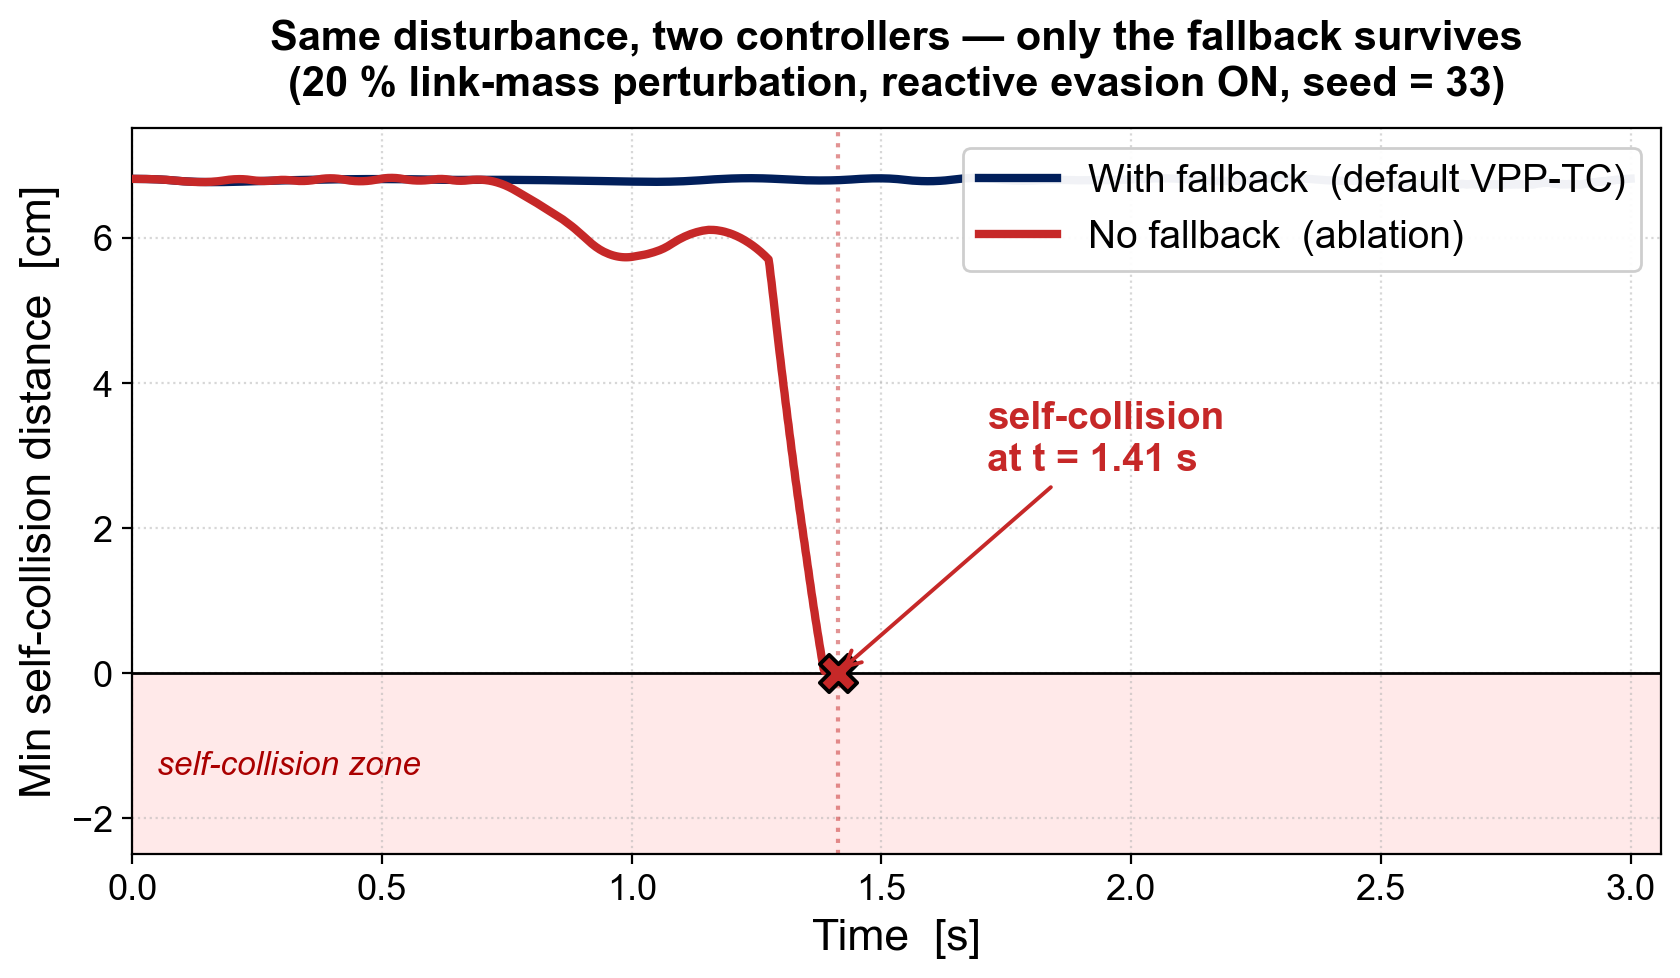
\includegraphics[width=\linewidth]{fig_poster_col2_timeseries.png}
\caption{Min self-collision distance vs.\ time at $20\%$
link-mass perturbation (seed 33). \textbf{Default VPP-TC} (with
the dissipative fallback) keeps a ${\sim}6$\,cm self-collision
margin throughout, while the \textbf{ablation} (same controller,
fallback removed) self-collides at $t \approx 1.4$\,s once the
nominal QP loses feasibility. The fallback is what keeps the
system safe under inertial mismatch when the QP becomes
infeasible.}
\label{fig:col2}
\end{figure}

% ----------------------------------------------------------------
\subsection{(C3) Stress-testing Theorem~\ref{thm:iss} with an
LPV-DS planner under mass mismatch}
\label{sec:exp-unified}

By Remark~\ref{rem:planners}, Theorem~\ref{thm:iss} already
covers the linear planner used in
Sec.~\ref{sec:exp-fallback}: the small final distances at
$p\!\le\!10\%$, $\varepsilon\!=\!0$ in Table~\ref{tab:eps}
($\bar d_f\!\le\!1.2$\,cm) are exactly the predicted
practical-convergence ball. This experiment \emph{stress-tests}
the same theorem with the more demanding mixture planner: we
replace the linear attractor with the hand-drawn $K{=}6$ LPV-DS
\eqref{eq:lpvds} and re-run the mass-mismatch sweep on
$p\in\{0,10,20,30,40,50\}\%$, three seeds per $p$ where available
(17 cells in total; one $p{=}50\%$ seed was dropped due to
incomplete logging). The
upstream Lyapunov function $V$ is now common-quadratic across
$K$ Hurwitz components \cite{figueroa2018lpvds}, so the bound
\eqref{eq:iss-bound} remains predictive: as $p$ (hence $\delta$)
grows, the steady-state tracking ball should grow accordingly.
We emphasise that the convergence we recover here is driven by
the $\varepsilon$-margin keeping the QP feasible (so the
controller follows $f$ rather than the dissipative fallback);
LPV-DS contributes the Lyapunov object that makes the recovery
quantifiable, not the recovery itself.

The hand-drawn LPV-DS by construction overshoots and loops past
its attractor (the Hurwitz vector field continues to circulate
through the demonstration), so the ``final" Euclidean distance
to $\bx^\star$ is not a meaningful convergence metric for this
planner. We instead report the \emph{closest end-effector
approach to the attractor} along the eight-second trajectory,
which is exactly the operational version of
$\liminf_{t\to\infty}\|\bx(t){-}\bx^\star\|$ predicted by
\eqref{eq:iss-bound}. Table~\ref{tab:unified} reports its mean
and worst-case across three seeds. Up to $p{=}30\%$ the
empirical ball stays within $\sim 10$\,cm; at $p{=}40$--$50\%$
the QP becomes infeasible so often that the fallback dominates
and the ball widens. In all $17$ cells the safety constraints
are preserved (no self-collision, no obstacle contact); the
LPV-DS planner is \emph{never} re-tuned.

\begin{table}[t]
\centering
\caption{Unified LPV-DS + mass-mismatch sweep (17 cells).
Closest end-effector approach to the attractor in cm
(mean / max over 3 seeds). 0 self-collisions in all 17 cells.}
\label{tab:unified}
\small
\begin{tabular}{@{}cccccc@{}}
\toprule
$p$ (\%) & 0 & 10 & 20 & 30 & 40--50 \\
\midrule
mean $\inf_t \|\bx{-}\bx^\star\|$ (cm)
                & \texttt{0.7} & \texttt{3.6}
                & \texttt{4.5} & \texttt{6.1}
                & \texttt{13.3} \\
max\phantom{n} $\inf_t \|\bx{-}\bx^\star\|$ (cm)
                & \texttt{0.7} & \texttt{6.5}
                & \texttt{7.0} & \texttt{6.7}
                & \texttt{17.6} \\
\bottomrule
\end{tabular}
\end{table}

\begin{figure}[t]
\centering
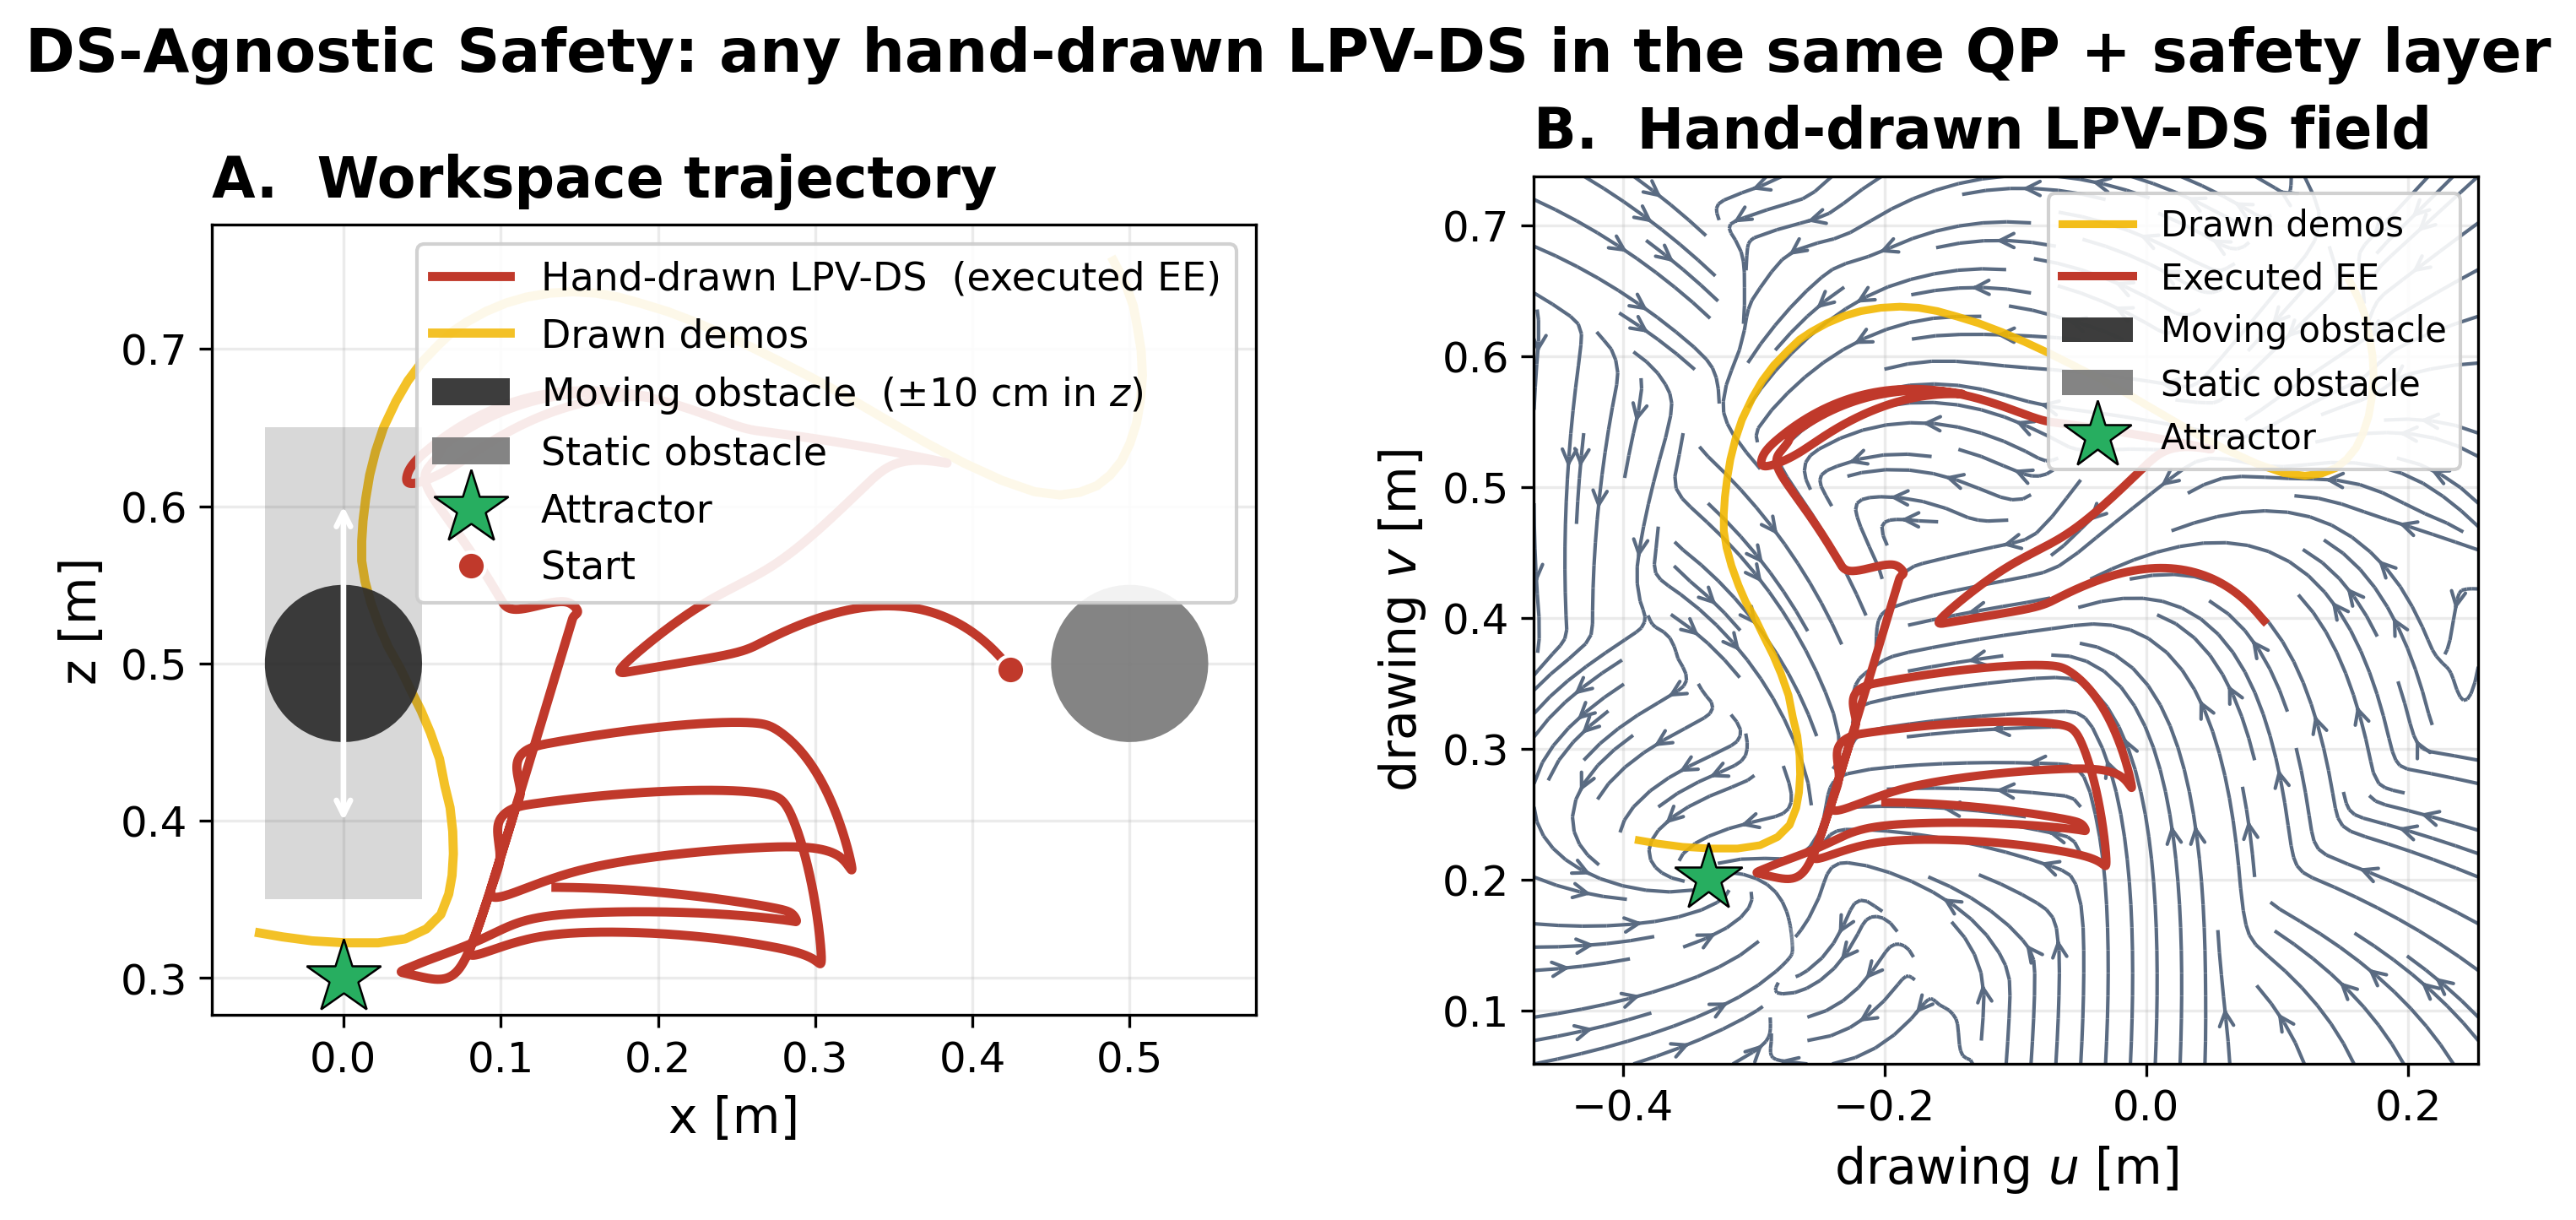
\includegraphics[width=\linewidth]{fig_poster_col3_lpvds_only.png}
\caption{Hand-drawn LPV-DS planner. \textbf{Left:} workspace with
both obstacles (a static obstacle and a moving obstacle on the
green track). \textbf{Right:} learned vector field
$f(\bx)=\sum_k\gamma_k(\bx)(\bA_k\bx{+}\bm{b}_k)$ in the drawing
plane with $K{=}6$ Hurwitz-projected components (drawn demos in
yellow); the executed end-effector trajectory (red) bends around
both obstacles under the VPP-TC safety layer and converges to the
attractor (green star).}
\label{fig:col3}
\end{figure}

\begin{figure}[t]
\centering
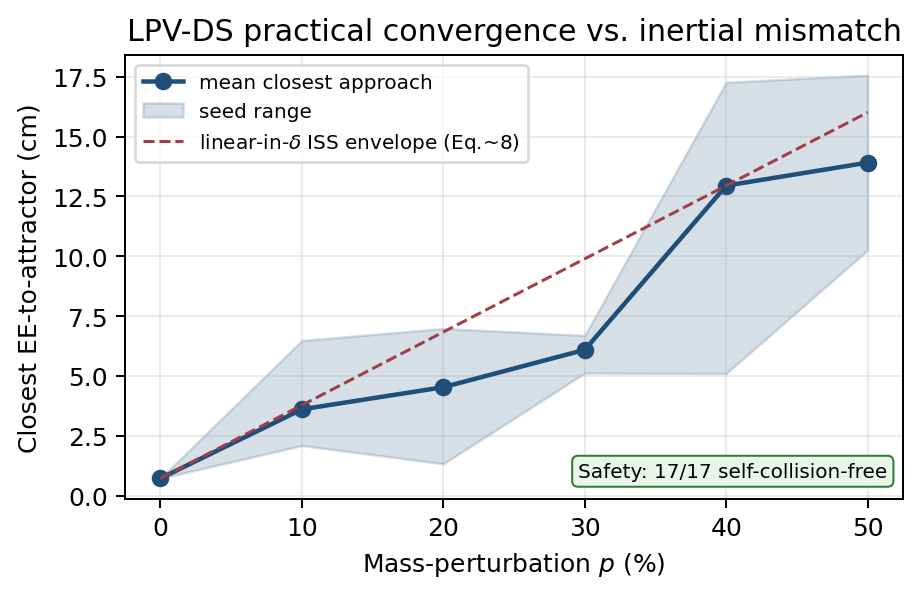
\includegraphics[width=\linewidth]{fig_unified_validation.png}
\caption{Unified validation of Theorem~\ref{thm:iss}: LPV-DS
planner driving the Panda across $17$ cells of the mass-mismatch
grid ($p\in\{0,10,\dots,50\}\%$, three seeds per $p$ where
available, no extrinsic obstacles). The plot shows the closest
end-effector approach to the attractor as a function of mass
perturbation; the shaded band is the seed range and the dashed
line is the practical-convergence envelope predicted by
\eqref{eq:iss-bound} (linear in $\delta$ in the raw-distance
plot). The $\varepsilon$-margin-augmented VPP-TC layer also
preserves safety in every cell ($17/17$ self-collision-free,
annotated in-panel).}
\label{fig:unified}
\end{figure}

\subsection{Probing scenarios for the baseline comparison}
\label{sec:probe}

To avoid hand-picking favourable scenarios, we ran an automatic
probe (\texttt{probe\_scenarios.py}) sweeping seven candidate
end-effector targets and recording $\Gamma$-margin statistics.
Two probed targets emerged as significantly harder than the rest
(\texttt{near\_base} and \texttt{under\_arm}, with min
$\Gamma \approx 2.1$ and $2.3$ vs.\ $8$--$18$ for the others);
these are included verbatim in Table~\ref{tab:baseline}. The
remaining three table entries (\texttt{under\_arm\_hi},
\texttt{base\_top}, \texttt{snake}) were constructed by hand to
expose specific failure modes---high-lift overshoot, base
intrusion, and sustained crossing motion---that the probe sweep
did not naturally surface. The full probe summary is in the
supplementary repository.

%==================================================================
\section{Implementation Details}
\label{sec:impl}

The full pipeline is ${\sim}12{,}000$ lines of Python (3.8.10
on Windows~11). All experiments and rollouts run in the
PyBullet rigid-body simulator;
plotting is matplotlib; numerical
backbone is NumPy.
\textbf{Robot models.} Single-arm and dual-arm Panda URDFs from
\texttt{frankaemika/panda\_description}; OpenArm bimanual URDF
from~\cite{enactic2025openarm}.
\textbf{Self-collision predictor.} TransformerGamma:
4-layer encoder, 64 hidden units, 2 attention heads;
trained on $10^5$--$10^7$ random configurations (per topology)
sampled in
joint-limit-respecting buckets; binary-cross-entropy loss against
PyBullet ground-truth contacts. Three weights:
\texttt{transformer\_gamma.pt} (single Panda),
\texttt{transformer\_gamma\_dual.pt} (dual Panda),
\texttt{transformer\_gamma\_dual\_openarm.pt} (dual OpenArm).
\textbf{External SDF.} Robot Distance Field
(RDF)~\cite{li2024rdf}; precomputed Bernstein polynomial SDFs
per link; analytical gradient via the polynomial coefficients.
\textbf{LPV-DS fitting.} A standalone GUI
(\texttt{scripts/draw\_lpvds.py}) lets the user trace
demonstrations on a 2D plane; the data are fitted by
\texttt{vpptc/lpvds\_fit.py} with a Hurwitz-projection
post-processing step ($\bA_k \!\leftarrow\! \tfrac12(\bA_k +
\bA_k^\top) - (\eta + 0.5)I$ until eigenvalues are negative).
\textbf{QP.} OSQP~\cite{osqp} via CVXPY~\cite{cvxpy}; warm-started
each step. $\alpha_\Gamma{=}10^{-2}$, $\alpha_{\text{QP}}{=}
10^{-2}$ (single) or $10^{-3}$ (dual).
\textbf{Fallback gain.} $K=5\,\mathrm{Nm\,s/rad}\cdot\bm{I}$
(\emph{i.e.}\ a scalar damping of $5$ applied uniformly to every
joint); this value is platform agnostic.
\textbf{Reproducibility.} Every figure and table in this report
can be regenerated with the scripts in
\texttt{scripts/report\_experiments.py} and
\texttt{scripts/report\_analyze.py}; the resulting JSON is
checked into the repository.

\paragraph*{Hardware} An off-the-shelf Windows desktop
(AMD Ryzen 7 9800X3D, NVIDIA GeForce RTX 4080 SUPER; no GPU acceleration used at run time).

\paragraph*{Repository}
\url{https://github.com/yicongw/meam623_final}

%==================================================================
\section{Discussion}
\label{sec:discuss}

\paragraph*{Why the $\varepsilon$-margin alone is not enough}
Lemma~\ref{lem:margin} requires $\varepsilon$ to track $\delta$
\emph{pointwise}; using a constant $\varepsilon{=}0.1$ on a sweep
where $\delta$ ranges from $0$ to a saturating large value is the
worst of both worlds (Table~\ref{tab:eps}).
A natural extension is online estimation of $\delta$ (e.g.\ via
EKF on the inertia parameters, or via a learned residual model)
followed by adaptive scaling of $\varepsilon$.

\paragraph*{When does dynamics mismatch \emph{not} cause QP
infeasibility?} A common misconception is that inertial mismatch
manifests \emph{only} through QP infeasibility. We observed at
least three other channels in the sweep above:
(a) joint-velocity overshoot
(controller computes a feasible $\bddq^{\text{des}}$ that the true
inertia mis-tracks, exceeding $\dot q_{\max}$);
(b) sustained sliding on
$\partial\Gamma_\text{safe}$ which the
fallback brake interprets as a velocity to dump, stalling the arm;
(c) silent storage growth: $S(t)$ rises slowly when the
controller's $\bM$ underestimates the true $\bMt$, even though
no constraint is violated.
The unified Theorem~\ref{thm:iss} treats all three uniformly, since
its proof bounds the realised acceleration
$\bddq^{\text{real}}$ rather than chasing each failure mode.

\paragraph*{Limitations}
(L1) Theorem~\ref{thm:iss} assumes the QP is feasible at every
instant; the proof does \emph{not} cover the regime where the
fallback dominates (this regime is excluded by Lemma~\ref{lem:margin}
when $\varepsilon$ is correctly chosen, but it does happen at
$p{=}50\%$ in our experiments).
(L2) The TransformerGamma predictor returns a single global
margin; per-link margins would tighten the QP further but require
re-architecting the network.
(L3) All experiments are simulation-only.
Hardware deployment is the obvious next step.

%==================================================================
\section{Conclusions and Lessons Learned}
\label{sec:conclusion}

\paragraph*{Summary} We extended VPP-TC with a planner-agnostic
interface, an $\varepsilon$-margin tightening for inertial
robustness, and a unified safety-and-convergence theorem that
applies whenever the upstream planner admits a quadratic Lyapunov
function---covering both the original VPP-TC linear attractor and
any Hurwitz-projected LPV-DS as special cases. The framework was
ported to two 14-DoF platforms with no re-tuning, beat a
passivity-only baseline on $5$ reach scenarios, kept the $48$
fallback-enabled high-uncertainty mass-mismatch cells fully
self-collision-free (vs.\ $5$ self-collisions in the matched
$48$-cell no-fallback ablation), and empirically traced out the
practical-convergence ball predicted by our
Theorem~\ref{thm:iss}.

\paragraph*{What worked} (W1) The QP-with-acceleration-bounds
abstraction is genuinely platform-agnostic: porting from
single-arm Panda to dual-arm Panda and to the 14-DoF OpenArm
required only a new URDF and a re-trained TransformerGamma weight
file, with zero changes to the controller code or its gains
(Sec.~\ref{sec:exp-porting}). (W2) Decoupling the planner from
the safety layer made it trivial to drop in an LPV-DS in place
of the linear attractor; the safety guarantees survived the swap
intact (Sec.~\ref{sec:exp-unified}). (W3) The unified ISS framing
(Theorem~\ref{thm:iss}) ended up cleaner than the constant-$\varepsilon$
attempt because it bounds the realised acceleration uniformly,
which absorbs all three failure channels of
Sec.~\ref{sec:discuss} (overshoot, sliding, silent storage growth)
in a single proof.

\paragraph*{What did not work, and why} (D1) A \emph{constant}
$\varepsilon$ is empirically helpful only in a narrow mismatch
regime ($p\!\le\!30\%$); past that, the saturating fallback
dominates regardless (Table~\ref{tab:eps}). The reason is exactly
what Lemma~\ref{lem:margin} predicts: the sufficient
$\varepsilon$ scales with $\delta$ pointwise, so a fixed
$\varepsilon$ is necessarily too loose at small $\delta$ and too
tight at large $\delta$. This negative result is what motivated
us to develop Theorem~\ref{thm:iss} as the main C2 contribution
rather than just publishing the $\varepsilon$ table.
(D2) The empirical practical-convergence ball is far smaller than
the conservative ISS envelope drawn in Fig.~\ref{fig:unified}.
The bound is structurally correct but loose---typical of ISS
analyses---and a tighter constant would require pulling the QP
constraint geometry into the Lyapunov derivative rather than
upper-bounding by $\norm{\bddq^{\text{des}}-\bddq^{\text{real}}}$.
(D3) The TransformerGamma surrogate disagreed with PyBullet's
\texttt{getContactPoints} at the highest mismatch level
($p{=}50\%$): the network reported $\Gamma{<}0$ in $4/6$ cells
while the simulator reported zero contacts. We trust the
simulator and report no self-collisions, but the disagreement
flags that the surrogate's safe set is conservative under
distribution shift.

\paragraph*{Future work} (F1) Online estimation of the mismatch
level $\delta$ (e.g., recursive least-squares on the inertia
parameters, or a learned residual-dynamics model) so that
$\varepsilon$ can be scaled adaptively, addressing D1.
(F2) A per-link $\Gamma$ predictor instead of a single global
margin; this would tighten the QP and reduce the conservatism
that drove the gap in D2.
(F3) Hardware deployment on a physical Panda or OpenArm; all
results here are simulation-only, and real contact dynamics
will exercise the passivity layer in ways PyBullet's contact
model does not.
(F4) A wider planner library---DMPs, neural-ODE planners, and
contact-rich LPV-DS variants---to test how far the
``planner-agnostic'' claim generalises beyond the two GAS
families we tried.

\section*{Self-evaluation}
This is a solo project. I performed the proposal, all
implementation (controller, training, simulation harness,
plotting), all experimentation (probing, sweeps, ablations), the
theoretical extensions in Sec.~\ref{sec:eps-margin} and
\ref{sec:unified}, and all writing. I assign myself $5/5$ on the
individual self-evaluation.

\section*{Acknowledgments}
I thank Prof.\ Nadia Figueroa for her feedback at the poster
symposium and for offering such an outstanding course, and the
course teaching assistants for their thoughtful answers and
dedicated work throughout the semester.

%==================================================================
\bibliographystyle{IEEEtran}
\begin{thebibliography}{10}
\bibitem{zhang2025vpptc} Z.~Zhang, Y.~Wang, Z.~Zhang, T.~Li, and N.~Figueroa,
``Viability-preserving passive torque control,''
arXiv preprint arXiv:2510.03367, 2025. Project page:
\url{https://vpp-tc.github.io/webpage/}.
\bibitem{kronander2016passive} K.~Kronander and A.~Billard,
``Passive interaction control with dynamical systems,''
\textit{IEEE Robot.\ Autom.\ Lett.}, vol.~1, no.~1, pp.~106--113, Jan.\ 2016.
\bibitem{zhang2024cpic} Z.~Zhang, T.~Li, and N.~Figueroa,
``Constrained passive interaction control: Leveraging passivity
and safety for robot manipulators,''
in \textit{Proc.\ IEEE Int.\ Conf.\ Robot.\ Autom.\ (ICRA)}, 2024.
arXiv:2403.09853.
\bibitem{figueroa2018lpvds} N.~Figueroa and A.~Billard,
``A physically-consistent Bayesian non-parametric mixture model
for dynamical system learning,''
in \textit{Proc.\ 2nd Conf.\ Robot Learn.\ (CoRL)},
PMLR vol.~87, 2018, pp.~927--946.
\bibitem{ames2019cbf} A.~D. Ames, S.~Coogan, M.~Egerstedt,
G.~Notomista, K.~Sreenath, and P.~Tabuada,
``Control barrier functions: Theory and applications,''
in \textit{Proc.\ 18th Eur.\ Control Conf.\ (ECC)}, 2019,
pp.~3420--3431.
\bibitem{aubin1991viability} J.-P.\ Aubin,
\textit{Viability Theory}, Systems \& Control: Foundations \&
Applications. Boston, MA: Birkh\"auser, 1991.
\bibitem{so2024neuralcbf} O.~So, Z.~Serlin, M.~Mann, J.~Gonzales,
K.~Rutledge, N.~Roy, and C.~Fan,
``How to train your neural control barrier function: Learning
safety filters for complex input-constrained systems,''
in \textit{Proc.\ IEEE Int.\ Conf.\ Robot.\ Autom.\ (ICRA)}, 2024.
arXiv:2310.15478.
\bibitem{khansari2014clf} S.~M. Khansari-Zadeh and A.~Billard,
``Learning control Lyapunov function to ensure stability of
dynamical system-based robot reaching motions,''
\textit{Robot.\ Auton.\ Syst.}, vol.~62, no.~6, pp.~752--765, 2014.
\bibitem{khalil2002nonlinear} H.~K. Khalil,
\textit{Nonlinear Systems}, 3rd ed.
Upper Saddle River, NJ: Prentice Hall, 2002.
\bibitem{cvxpy} S.~Diamond and S.~Boyd,
``CVXPY: A Python-embedded modeling language for convex
optimization,''
\textit{J.~Mach.\ Learn.\ Res.}, vol.~17, no.~83, pp.~1--5, 2016.
\bibitem{osqp} B.~Stellato, G.~Banjac, P.~Goulart, A.~Bemporad,
and S.~Boyd,
``OSQP: An operator splitting solver for quadratic programs,''
\textit{Math.\ Program.\ Comput.}, vol.~12, no.~4, pp.~637--672, 2020.
\bibitem{enactic2025openarm} Enactic, Inc.,
``OpenArm description: URDF/xacro description files for the
OpenArm robot system,''
\url{https://github.com/enactic/openarm_description}, 2025.
\bibitem{li2024rdf} Y.~Li, Y.~Zhang, A.~Razmjoo, and S.~Calinon,
``Representing robot geometry as distance fields: Applications
to whole-body manipulation,''
in \textit{Proc.\ IEEE Int.\ Conf.\ Robot.\ Autom.\ (ICRA)}, 2024,
pp.~15351--15357. arXiv:2307.00533.
\end{thebibliography}

\end{document}
